%%%%%%%%%%%%%%%%%%%%%%%%%%%%%%%%%%%%%%%%%
% Make sure to set your name, legi number and url to the right git branch.
\newcommand{\hmwkAuthorName}{SILVAN WEDER} % Your name
\newcommand{\hmwkAuthorLegi}{13-914-643} % Your name
\newcommand{\hmwkGitBranch}{$13-914-643/$1_locally_linear_embedding} % Your name
%
%%%%%%%%%%%%%%%%%%%%%%%%%%%%%%%%%%%%%%%%%

%----------------------------------------------------------------------------------------
%	PACKAGES AND OTHER DOCUMENT CONFIGURATIONS
%	Skip this
%----------------------------------------------------------------------------------------

\documentclass{article}


\usepackage{caption}
\usepackage{amsmath}
\usepackage{amsfonts}
\usepackage{mathtools}
\usepackage{fancyhdr} % Required for custom headers
\usepackage{lastpage} % Required to determine the last page for the footer
\usepackage{extramarks} % Required for headers and footers
\usepackage{graphicx} % Required to insert images
\usepackage{lipsum} % Used for inserting dummy 'Lorem ipsum' text into the template

% Margins
\topmargin=-0.45in
\evensidemargin=0in
\oddsidemargin=0in
\textwidth=6.5in
\textheight=9.0in
\headsep=0.25in 

\linespread{1.1} % Line spacing

% Set up the header and footer
\pagestyle{fancy}
\lhead{\hmwkAuthorName} % Top left header
\chead{\hmwkClass\ \hmwkTitle} % Top center header
\rhead{\firstxmark} % Top right header
\lfoot{\lastxmark} % Bottom left footer
\cfoot{} % Bottom center footer
\rfoot{Page\ \thepage\ of\ \pageref{LastPage}} % Bottom right footer
\renewcommand\headrulewidth{0.4pt} % Size of the header rule
\renewcommand\footrulewidth{0.4pt} % Size of the footer rule

\setlength\parindent{0pt} % Removes all indentation from paragraphs

%----------------------------------------------------------------------------------------
%	DOCUMENT STRUCTURE COMMANDS
%	Skip this
%----------------------------------------------------------------------------------------

% Header and footer for when a page split occurs within a problem environment
\newcommand{\enterProblemHeader}[1]{
\nobreak\extramarks{#1}{#1 continued on next page\ldots}\nobreak
\nobreak\extramarks{#1 (continued)}{#1 continued on next page\ldots}\nobreak
}

% Header and footer for when a page split occurs between problem environments
\newcommand{\exitProblemHeader}[1]{
\nobreak\extramarks{#1 (continued)}{#1 continued on next page\ldots}\nobreak
\nobreak\extramarks{#1}{}\nobreak
}

\setcounter{secnumdepth}{0} % Removes default section numbers
\newcounter{homeworkProblemCounter} % Creates a counter to keep track of the number of problems

\newcommand{\homeworkProblemName}{}
\newenvironment{homeworkProblem}[1][Problem \arabic{homeworkProblemCounter}]{ % Makes a new environment called homeworkProblem which takes 1 argument (custom name) but the default is "Problem #"
\stepcounter{homeworkProblemCounter} % Increase counter for number of problems
\renewcommand{\homeworkProblemName}{#1} % Assign \homeworkProblemName the name of the problem
\section{\homeworkProblemName} % Make a section in the document with the custom problem count
\enterProblemHeader{\homeworkProblemName} % Header and footer within the environment
}{
\exitProblemHeader{\homeworkProblemName} % Header and footer after the environment
}

\newcommand{\problemAnswer}[1]{ % Defines the problem answer command with the content as the only argument
\noindent\framebox[\columnwidth][c]{\begin{minipage}{0.98\columnwidth}#1\end{minipage}} % Makes the box around the problem answer and puts the content inside
}

\newcommand{\homeworkSectionName}{}
\newenvironment{homeworkSection}[1]{ % New environment for sections within homework problems, takes 1 argument - the name of the section
\renewcommand{\homeworkSectionName}{#1} % Assign \homeworkSectionName to the name of the section from the environment argument
\subsection{\homeworkSectionName} % Make a subsection with the custom name of the subsection
\enterProblemHeader{\homeworkProblemName\ [\homeworkSectionName]} % Header and footer within the environment
}{
\enterProblemHeader{\homeworkProblemName} % Header and footer after the environment
}
   
%----------------------------------------------------------------------------------------
%	NAME AND CLASS SECTION
%	Skip this
%----------------------------------------------------------------------------------------

\newcommand{\hmwkTitle}{Locally Linear Embedding} % Assignment title
\newcommand{\hmwkDueDate}{Monday,\ March\ 6th,\ 2017} % Due date
\newcommand{\hmwkClass}{SLT coding exercise\ \#1} % Course/class
\newcommand{\hmwkClassTime}{Mo 16:15} % Class/lecture time
\newcommand{\hmwkClassInstructor}{} % Teacher/lecturer

%----------------------------------------------------------------------------------------
%	TITLE PAGE
%	Skip this
%----------------------------------------------------------------------------------------

\title{
\vspace{2in}
\textmd{\small{\hmwkClass}}\\
\textmd{\textbf{\hmwkTitle}}\\
\small{https://gitlab.vis.ethz.ch/vwegmayr/slt-coding-exercises}\\
\normalsize\vspace{0.1in}\small{Due\ on\ \hmwkDueDate}
%\vspace{0.1in}\large{\textit{\hmwkClassInstructor\ \hmwkClassTime}}
\vspace{3in}
}

\author{
\hmwkAuthorName\\
\hmwkAuthorLegi
}

\date{ } % Insert date here if you want it to appear below your name

\begin{document}

\maketitle

%----------------------------------------------------------------------------------------
%	TABLE OF CONTENTS
%	Skip this
%----------------------------------------------------------------------------------------

%\setcounter{tocdepth}{1} % Uncomment this line if you don't want subsections listed in the ToC

\newpage
\tableofcontents
\newpage

%----------------------------------------------------------------------------------------
%	SECTIONS
%	Now you are in the right hood
%----------------------------------------------------------------------------------------

\begin{homeworkProblem}[The Model]
The model section is intended to allow you to recapitulate the essential ingredients used in \hmwkTitle. Write down the \textit{necessary} equations to specify \hmwkTitle\ and and shortly explain the variables that are involved. This section should only introduce the equations, their solution should be outlined in the implementation section.\newline
Hard limit: One page
\vspace{10pt}

\problemAnswer{ 

In the Locally Linear Embedding problem, a set of $N$ points $\mathbf{x}_i$ with $D$ dimensions (e.g. $\mathbf{x}_i \in \mathbb{R}^D$). With the locally linear embedding the embedding of these points in a low dimensional space $\mathbb{R}^d$ is possible ($d << D$). In this low dimensional space each point $\mathbf{x}_i$ is represented by a point $\mathbf{y}_i \in \mathbb{R}^d$. 
\\
\\
The formulas for the implementation of the locally linear embedding are originally derived from its reconstruction error in this problem. Therefore, the reconstruction error is presented first.

\begin{equation}
\label{reconError}
\mathcal{E}\left(\mathbf{W}\right) =  \sum_{i} {\| \mathbf{x}_i - \sum_{j} w_{ij}\mathbf{x}_j\|^2}
\end{equation}

The points $\mathbf{x}_j$ are the $j$ closest neighbors of the point $\mathbf{x}_i$ and $w_{ij}$ are the weights, that correspond to each of this neighbors.
\\
\\ 
Then the reconstruction error is minimized using the constraint $\sum_j{w_{ij}} = 1$. This minimization yields the equation for the weights that give the optimal reconstruction with respect to the minimum of the reconstruction error given in \ref{reconError}.

\begin{equation}
\label{wij}
w_{ij} = \frac{\sum_{k}{C_{jk}^{(i)-1}}}{\sum_{lk}{C_{lk}^{(i)-1}}}
\end{equation}

The matrix $\mathbf{C}^{(i)}$ has the elements $C_{jk}^{(i)} = (\mathbf{x}_i - \mathbf{x}_j)^T(\mathbf{x}_i - \mathbf{x}_k)$ and $\mathbf{C}^{(i)-1}$ is its inverse.
\\
\\
Having now the weights $\mathbf{W}$, one can define the embedding error for the new points $\mathbf{y}_i \in \mathbb{R}^d$.

\begin{equation}
\label{embError}
\mathcal{E}\left(\mathbf{y}_1,...,\mathbf{y}_N \right) = \sum_i {\| \mathbf{y}_i - \sum_j{w_{ij}\mathbf{y}_j}\|^2}
\end{equation}

This equation \ref{embError} can also be written as

\begin{equation}
\mathcal{E}\left(\mathbf{y}_1,...,\mathbf{y}_N \right) = \sum_k{\mathbf{u}_k^T \mathbf{M}\mathbf{u}_k}
\end{equation}

where $\mathbf{u}_k = \left(y_{1k},...,y_{Nk}\right)$ for $k = 1,...,d$ and $M = \left(\mathbb{I}-\mathbf{W}\right)^T\left(\mathbb{I}-\mathbf{W}\right)$. It can be shown that the u's are found with the computation of the eigenvectors of $\mathbf{M}$. The correct u's are the ones that are associated with the smalles $d+1$ eigenvalues skipping the one with eigenvalue $0$.
}
\end{homeworkProblem}
\clearpage

%----------------------------------------------------------------------------------------
\begin{homeworkProblem}[The Questions]
This is the core section of your report, which contains the tasks for this exercise and your respective solutions. Make sure you present your results in an illustrative way by making use of graphics, plots, tables, etc. so that a reader can understand the results with a single glance. Check that your graphics have enough resolution or are vector graphics. Consider the use of GIFs when appropriate.\newline
Hard limit: Two pages

\begin{homeworkSection}{(a) Get the data}
For this exercise we will work with the MNIST data set. In order to learn more about it and download it, go to http://yann.lecun.com/exdb/mnist/.
\end{homeworkSection}

\begin{homeworkSection}{(b) Locally linear embedding}
Implement the LLE algorithm and apply it to the MNIST data set. Provide descriptive visualizations for 2D \& 3D embedding spaces. Is it possible to see clusters?
\end{homeworkSection}

\begin{homeworkSection}{(c) Cluster structure}
Investigate the cluster structure of the data. Can you observe block structures in the $M$ matrix (use matrix plots)? Also plot the singular values of $M$. Do you notice something?
Can you think of ways to determine the optimal embedding dimension?
\end{homeworkSection}

\begin{homeworkSection}{(d) Nearest Neighbors}
Investigate the influence of the choice of how many nearest neighbors you take into account. Additionally, try different metrics to find the nearest neighbors (we are dealing with images!).
\end{homeworkSection}

\begin{homeworkSection}{(e) Linear manifold interpolation}
Assume you pick some point in the embedding space. How can you map it back to the original (high dimensional) space? Investigate how well this works for points within and outside the manifold (does it depend on the dimensionality of the embedding space?) Try things like linearly interpolating between two embedding vectors and plot the sequence of images along that line. What happens if you do that in the original space?
\end{homeworkSection}

\clearpage

\vspace{10pt}
\begin{homeworkSection}{(a) Get the data}

The MNIST data set is used for the Locally Linear Embedding problem. The data set has  $60000$ images of handwritten numbers from $0$ to $9$.

\begin{figure}[h]
\begin{minipage}[t]{ 0.45\textwidth}
\centering
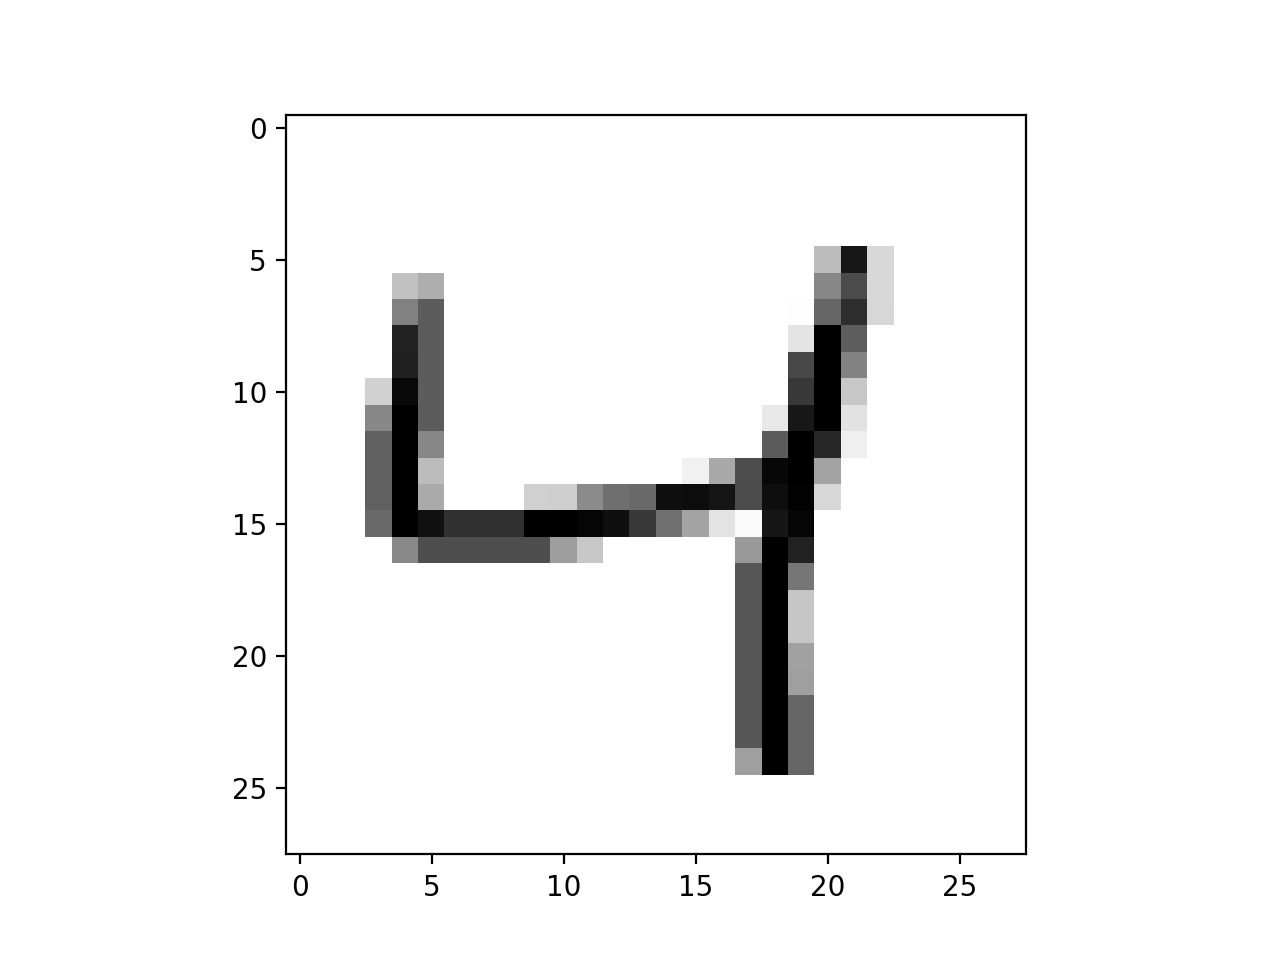
\includegraphics[scale=0.25]{Figures/example4.png}
\caption{Gray-scale image of number 4}
\end{minipage}
\begin{minipage}[t]{ 0.45\textwidth}
\centering
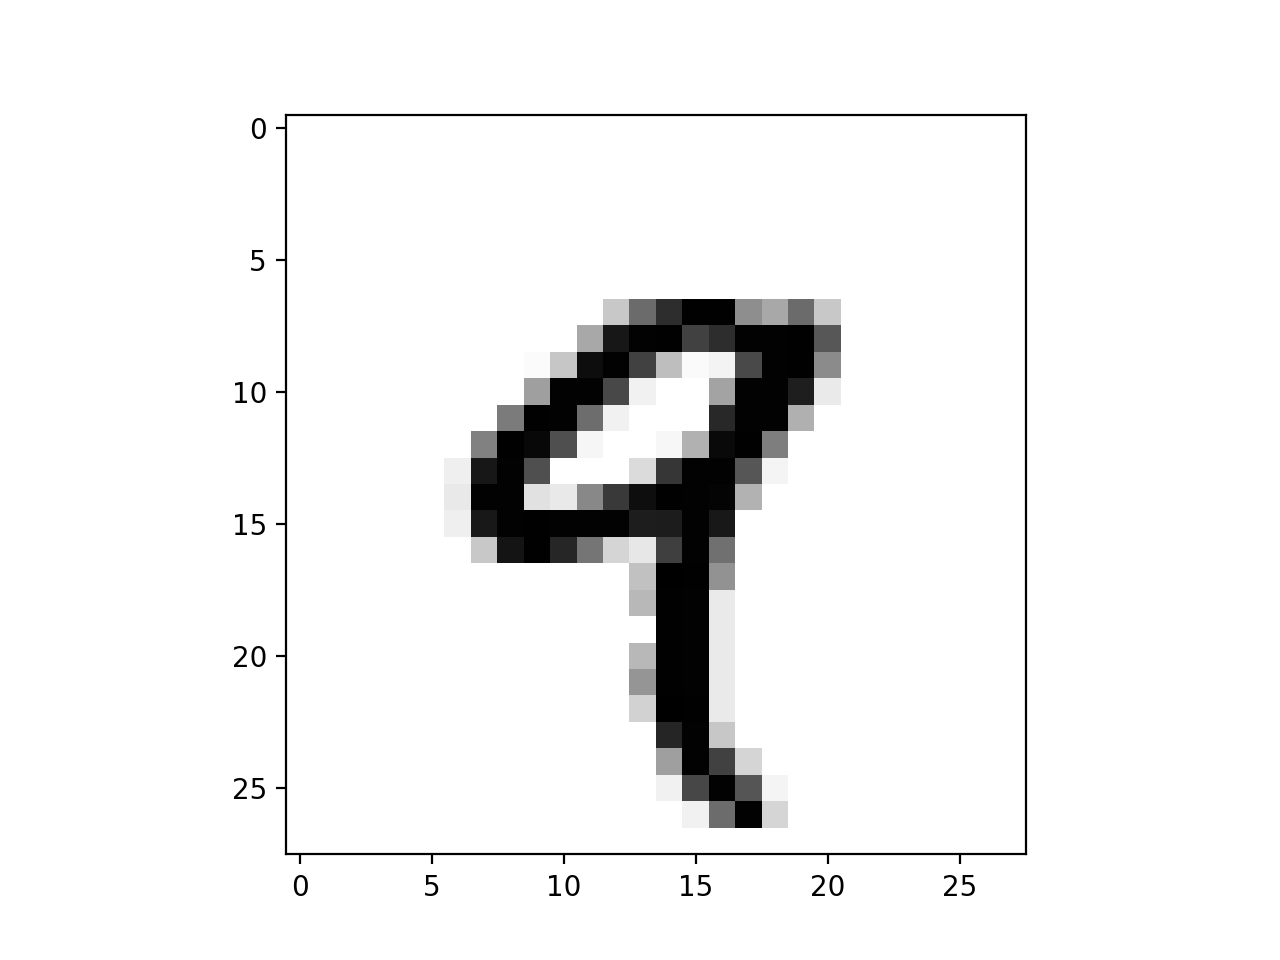
\includegraphics[scale=0.25]{Figures/example9.png}
\caption{Gray-scale image for number 9}
\end{minipage}
\end{figure}

\end{homeworkSection}

\begin{homeworkSection}{(b) Locally linear embedding}
The images of the handwritten figures are transformed into $D$-dimensional vectors and then embedded in a space of dimension $2$ and $3$. 

\begin{figure}[h]
\begin{minipage}[c]{ 0.45\textwidth}
\centering
\includegraphics[scale=0.4]{Plots/2D/Euclidean/2D_LLE_plot_c_2_n_9_m_euclidean.png}
\label{2DLLE}
\captionsetup{width=0.9\textwidth}
\caption{Locally linear embedding of 5000 MNIST images into a 2 dimensional space}
\end{minipage}
\begin{minipage}[c]{ 0.45\textwidth}
\centering
\includegraphics[scale=0.4]{Plots/3D/Euclidean/3D_LLE_plot_c_3_n_9_m_euclidean.png}
\label{3DLLE}
\captionsetup{width=0.9\textwidth}
\caption{Locally linear embedding of 5000 MNIST images into a 2 dimensional space}
\end{minipage}
\end{figure}

In figures 3 and 4, the LLE into 2- or 3-dimensional space is shown. One can clearly see the cluster of the different numbers in the MNIST sample. For this LLE, 9 neighbors have been used for the nearest neighbor computation and the Euclidean vector norm has been used as a metric.

\end{homeworkSection}

\begin{homeworkSection}{(c) Cluster structure}

In order to study the structure of the matrix $M$ that is used for the LLE, $M$ is plotted as it is shown in figure 5.

\begin{figure}[h]
\begin{minipage}[c]{0.45\textwidth}
\centering
\includegraphics[scale=0.3]{Plots/Matrixplot/matrixplot_M.png}
\label{Mplot}
\caption{Matrixplot of matrix $M$}
\end{minipage}
\begin{minipage}[c]{0.45\textwidth}
\centering
\includegraphics[scale=0.3]{Plots/Matrixplot/singularvalues.png}
\label{SingularValues}
\caption{Plot of singular values of matrix  $M$}
\end{minipage}
\end{figure}

In this plot, one can observe that the matrix M has a block-diagonal structure. For each number from $0$ to $9$ there is a corresponding block in the matrix. Looking at the singular values when the labels of the training data are sorted, one can easily see that the singular values are strictly decreasing. Therefore, I would propose to introduce a LLE with 10 coordinates (e.g. for each label one coordinate).  

\end{homeworkSection}

\begin{homeworkSection}{(d) Nearest Neighbors}

In order to analyze the influence of the number of neighbors chosen in the nearest neighbor computation, two plots with different numbers of neighbors are presented in figure 7 and 8.

\begin{figure}[h]
\begin{minipage}[c]{ 0.45\textwidth}
\centering
\includegraphics[scale=0.4]{Plots/2D/Euclidean/2D_LLE_plot_c_2_n_9_m_euclidean.png}
\label{nn7}
\caption{LLE with 7 neighbor points}
\end{minipage}
\begin{minipage}[c]{ 0.45\textwidth}
\centering
\includegraphics[scale=0.45]{Plots/2D/Euclidean/2D_LLE_plot_c_2_n_20_m_euclidean.png}
\label{nn15}
\caption{LLE with 20 neighbor points}
\end{minipage}
\end{figure}

From these plots, it can be derived that the an increasing number of neighbors used in the computation does not improve the structure of the clusters in the result. However, a number of neighbors that is too low is also not recommendable because then, the clusters are seperable.

If one changes the metric that is used for the nearest neighbor computation, the results look quite similar. Although there is a slight rotation in the plots around the center of the plot.

\end{homeworkSection}

\begin{homeworkSection}{(e) Linear manifold interpolation}

The reconstruction of points from inside the manifold works quite well as it is shown in the images below. However, if the point is not part of the manifold, the reconstruction is not working well anymore. Although, there are still some features of a number visible, it is hard to tell what number it is.

\begin{figure}[h]
\begin{minipage}[t]{ 0.45\textwidth}
\centering
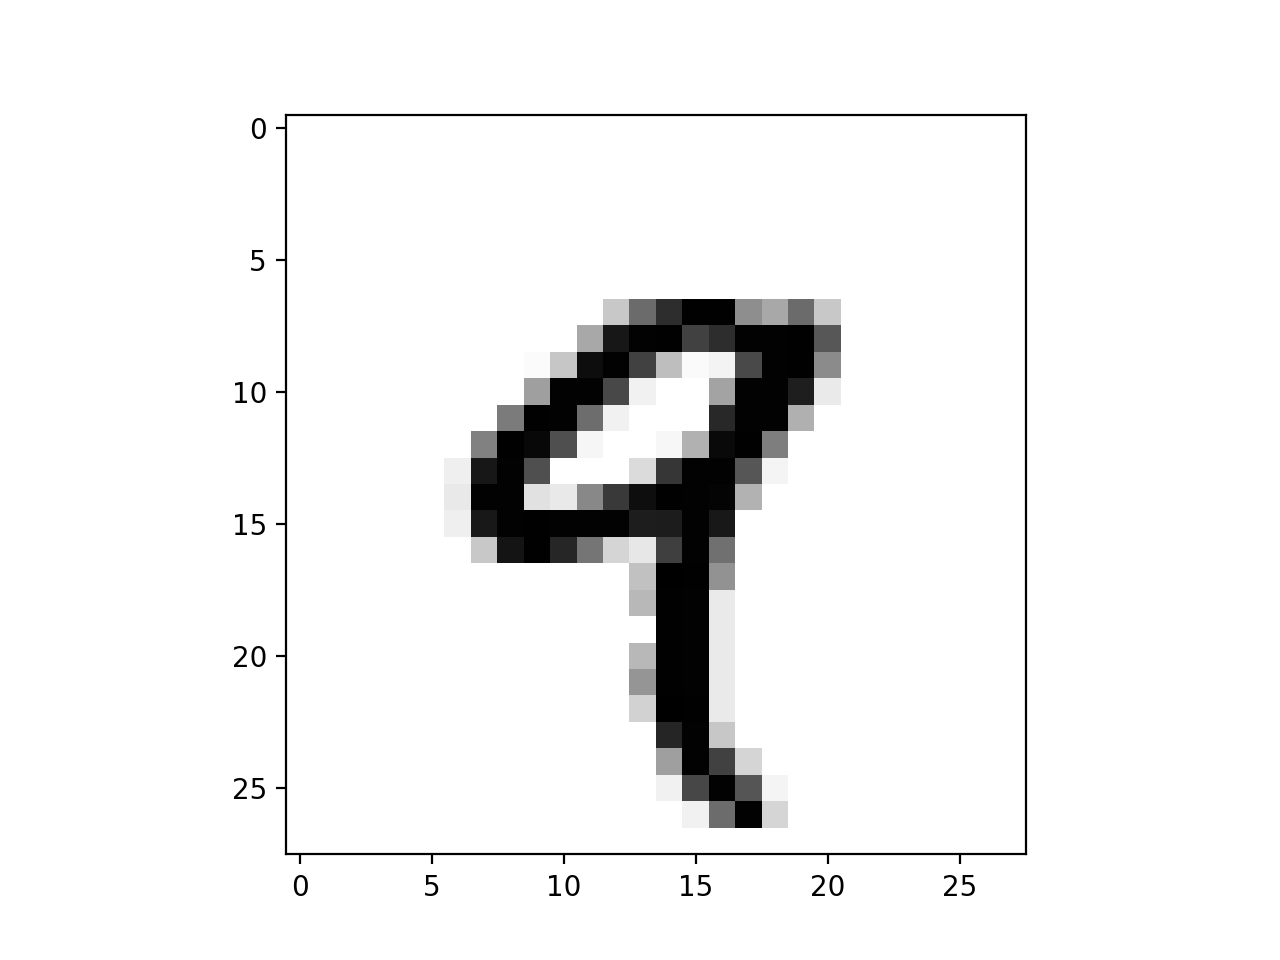
\includegraphics[scale=0.25]{Figures/example9.png}
\caption{Original gray-scale image}
\end{minipage}
\begin{minipage}[t]{ 0.45\textwidth}
\centering
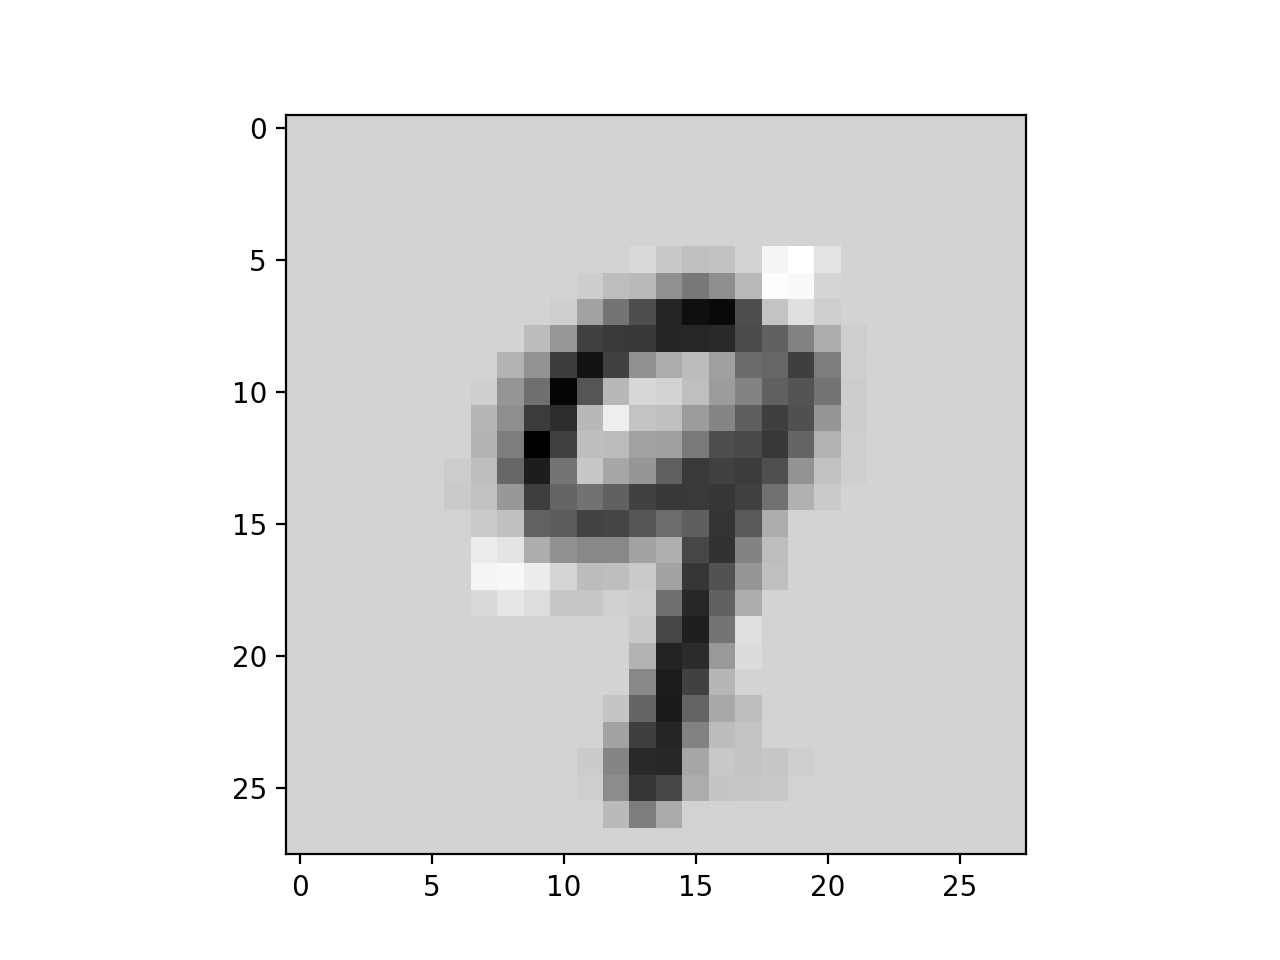
\includegraphics[scale=0.25]{Figures/reconstructed9.png}
\caption{Reconstructed gray-scale image from the embedded space}
\end{minipage}
\end{figure}

\end{homeworkSection}



\end{homeworkProblem}


\clearpage

%----------------------------------------------------------------------------------------
\begin{homeworkProblem}[The Implementation]
In the implementation section you give a concise insight to the practical aspects of this coding exercise. It mainly mentions the optimization methods used to solve the model equations. Did you encounter numerical or efficiency problems? If yes, how did you solve them?
Provide the link to your git branch of this coding exercise.\newline
Hard limit: One page

\vspace{10pt}
\problemAnswer{

For this problem I mainly used the numpy and scipy libraries for python. The LLE algorithm I implemented from scratch. However, for the nearest neighbors computation I used the NearestNeighbors class from the sklearn library in order to achieve a proper efficiency of my code. As the nearest neighbors computation and the solver for the eigenvalues/eigenvectors scale with $N^2$, the code was efficient enough to run on my computer. However, I restricted the number of data to 5000 in order to get results in a reasonable time.
\\
\\
\textbf{Algorithm}

\begin{enumerate}
\item Nearest Neighbor Computation using NearestNeighbors-functions from the sklearn library. For the Computation the kd-tree algorithm is used.

\item Computation of the weights using simple linear algebra tools from numpy.

\item Computation of matrix $\textbf{M}$ and solving for the $d+1$ smallest eigenvalues. For the eigenvalue compuation the function $eigh()$ has been used.

\end{enumerate}
\textbf{Git Branch}
13-914-643/1\_ locally\_ linear\_ embedding


}
\end{homeworkProblem}
\clearpage

%----------------------------------------------------------------------------------------
\begin{homeworkProblem}[Your Page]
Your page gives you space to include ideas, observations and results which do not fall into the categories provided by us. You can also use it as an appendix to include things which did not have space in the other sections.\newline
No page limit.

\vspace{10pt}
\problemAnswer{ % Answer


}
\end{homeworkProblem}
\clearpage

\end{document}

